\documentclass[aps,pre,twocolumn,superscriptaddress,floatfix,nofootinbib]{revtex4-2}

\usepackage{amsmath,amssymb}
\usepackage{graphicx}
\usepackage{bm}
\usepackage[colorlinks=true,allcolors=blue]{hyperref}

\begin{document}

\title{Phase diagram of networks grown with triadic closure rules}

\author{Alexei Vazquez}
\email{alexei@nodeslinks.com}
\affiliation{Nodes \& Links Ltd, Salisbury House, Station Road, Cambridge, CB1 2LA, UK}

\date{\today}

\begin{abstract}
We map numerically, up to $n=10^7$ nodes, the phase diagram of a network grown
by four independent processes: nodes arrive at rate
$\alpha_+$ and attach to a random node, random nodes are deleted at rate
$\alpha_-<\alpha_+$, open triads close at rate $\beta_+$, and closed triads open
at rate $\beta_-$. For $\beta_-\ge\beta_+$ the triangles form a critical or
subcritical queue, and the network is a tree with a Poisson-like degree tail.
For $\beta_+>\beta_-$ the outcome depends on how the open triad is found. We
take as order parameter the fraction $P_\triangle$ of triangles in the largest
cluster of triangles that share links. When triads are drawn uniformly from the
whole network, the closure links concentrate on a vanishing fraction of the
nodes. Without opening they form a near-clique of about $\sqrt n$ nodes that
holds nearly all the triangles, and this condensate survives node deletion as a
steady state rebuilt from young nodes. Opening thins it. At one net closure
link per arrival and beyond a turnover $\beta_-/\beta_+$ between $0.76$ and
$0.78$, the triangles stop percolating up to $n=10^7$ nodes, although the
closure links still concentrate on the nodes of highest degree; whether this
dispersed regime is a phase or a long crossover remains open. Deletion moves
the boundary towards $\beta_-=\beta_+$. Closure within a node's neighbourhood
never condenses.
\end{abstract}

\maketitle

%=====================================================================
\section{Introduction}

Triadic closure, a link forming between two nodes that share a neighbour, is
the mechanism behind the high clustering of social networks
\cite{granovetter1973,davidsen2002,holme2002,vazquez2003,toivonen2006,jackson2007}.
In an evolving university e-mail network, pairs two steps apart were about 30
times more likely to form a tie than pairs three steps apart, and the
probability of a new tie grew with the number of common contacts
\cite{kossinets2006}. In dynamic online networks such as Digg and Facebook wall
posts the growth is consistent with a linear dependence on that number
\cite{ahmadian2021}, which is what follows when every open triad closes at the
same rate, as under rule (w) below. This evidence concerns the rate at which a
pair closes; it does not test the rate at which a node introduces its friends,
which under rule (w) grows as the square of its degree and feeds the hubs of
Sec.~\ref{sec:condensed}.
In the local-search model $LS(n,\ell)$ \cite{vazquez2001,vazquez2003,book} with
$\ell=1$ a newcomer picks a random node $j$, links to it and to a random
neighbour of $j$. Every arrival closes one triangle, so arrival and closure are
the same event, and no link is ever lost.

In a social system these are separate processes. People join and leave at
their own rates, acquaintances are introduced to each other at another, and
ties lapse at yet another. We therefore let four processes run side by side:
arrival at rate $\alpha_+$, deletion of a node at rate $\alpha_-$, closure of an
open triad at rate $\beta_+$, and opening of a closed triad, the reverse of
closure, at rate $\beta_-$. Meetings biased towards pairs with mutual friends,
combined with the decay of unrenewed ties, give clustered networks with strong
communities \cite{jin2001}, and growth by triadic closure alone generates
communities, which heterogeneous fitness replaces with a few superhubs
\cite{bianconi2014}. On a fixed population, link creation through friends of
friends balanced by random decay gives a discontinuous transition between a
sparse and a dense society \cite{marsili2004}, and a birth rate that grows with
the number of common neighbours gives bistability \cite{grindrod2012}. Closure
through a uniformly random wedge, our rule (w), defines the wedge picking model
of Ahmadian and Haddadan \cite{ahmadian2021}. They bounded the growth of a
vertex's degree over short time windows on a fixed vertex set; we follow the
same step over long times in a growing network. Static
triadic closure on a fixed backbone is exactly solvable \cite{cirigliano2024},
and in the random triadic process the graph becomes complete above a sharp
threshold \cite{korandi2016}.

Growth changes the outcome. In a fixed population the dense and sparse states
compete globally; in a growing network nodes differ by age, the dense state
appears on a vanishing fraction of them, and bistability becomes
condensation.

Our results are the following. A stationary density requires total rates in
fixed ratio, and it fixes the mean degree; at $\beta_-=\beta_+$ the triangles
become a critical queue and the network a tree (Sec.~\ref{sec:density}). When
closure draws its triads from the whole network, the triangles condense, after
a plateau whose length grows quickly as the closure rate decreases, onto a
near-clique of about $\sqrt n$ nodes that survives node deletion
(Sec.~\ref{sec:condensed}). Opening thins the condensate into a sparse cluster
and, beyond a turnover of about $0.77$, stops the triangles from percolating up
to $n=10^7$, although closure links still gather on the hubs
(Secs.~\ref{sec:phase} and \ref{sec:hubfree}); we cannot exclude a later onset.
Closure rules that find the triad locally never condense
(Sec.~\ref{sec:local}). The mean field (Sec.~\ref{sec:meanfield}) misses all of
this, and communities are discussed in Sec.~\ref{sec:mixing}.

%=====================================================================
\section{The model}
\label{sec:model}

The network starts from a path of three nodes. With
$Z=\alpha_++\alpha_-+\beta_++\beta_-$, each event is an \emph{arrival} with
probability $\alpha_+/Z$, in which a new node links to a uniformly random node;
a \emph{deletion} with probability $\alpha_-/Z$, in which a uniformly random
node is removed with all its links; a \emph{closure} with probability
$\beta_+/Z$, in which an open triad $a$--$c$--$b$ ($a$, $b$ unlinked) gets the
link $(a,b)$; or an \emph{opening} with probability $\beta_-/Z$, in which a
closed triad loses the link $(a,b)$. Since $Z$ only sets the clock,
rates are measured in units of $\alpha_+$. We keep $\alpha_-<\alpha_+$ so that
the network grows; for $\alpha_->\alpha_+$ its size stays small.

How a triad is chosen defines the rule, and each closure rule has a
mirror-image opening rule. Under the \emph{random-triad} rule (w) an open
(closed) triad is drawn uniformly from the whole network. Every open triad
thus closes at the same rate, so an unlinked pair with $m$ common neighbours
links at a rate proportional to $m$, and a node with $k$ neighbours introduces
each of its $k(k-1)/2$ pairs at the same rate. The centre of an open triad has
weight $k_c(k_c-1)$, and opening removes a link with probability proportional
to its number of triangles, $t_e$. Under the \emph{random-potential-link} rule
(p), closure picks a uniformly random unlinked pair with a common neighbour,
whatever their number of common neighbours, and opening a uniformly random link
with $t_e\ge1$; we sample an open triad as in rule (w) and accept it with
probability $1/m$, where $m$ is the number of common neighbours of its pair, so
that every eligible pair is equally likely; in the dense core most draws are
rejected, which costs time but introduces no bias. Under the \emph{introducer} rule (c), a
random node with $k_c\ge2$ links (unlinks) two of its neighbours. Under the
\emph{friend-of-a-friend} rule (f), a random node $a$ walks $a\to j\to l$,
$l\ne a$, and links to (unlinks from) $l$. Rules (w) and (p) need a census of
the network; (c) and (f) use only a node and its neighbourhood. A selection
that does not qualify is repeated. A closure that finds no open triad becomes
an arrival, and an opening that finds no closed triad does nothing; for
$\beta_-<\beta_+$ this happens only in the first few events, and for
$\alpha_-=0.95\,\alpha_+$ in $4\times10^{-5}$ of the closures. Opening
never disconnects the network, since $a$ and $b$ stay joined through $c$;
deletion can. Rule (w) is the main object of this paper; rules (p), (c) and (f)
are compared with it in Sec.~\ref{sec:local}, with $LS(n,1)$, one node and two
links per step, as reference.

The simulation keeps adjacency lists, a hash set of links, and Fenwick trees
over the triad weights and, with opening, over the $t_e$. Triangle counts are
updated incrementally and were checked against full recounts. Each link is
tagged with the event that created it. A run stops when the network first holds
$n$ nodes, so runs with the same seed and different $n$ are stages of one
trajectory.

%=====================================================================
\section{Density and the first transition}
\label{sec:density}

Write $r_\pm=\beta_\pm/\alpha_+$ for the number of closures and openings per
arrival, and
\begin{equation}
  \Delta=r_+-r_-=\frac{\beta_+-\beta_-}{\alpha_+}
  \label{eq:Delta}
\end{equation}
for the net closure per arrival, the links that closure adds, net of opening,
per arrival.
A deletion removes a node and, on average, $\langle k\rangle$ links. If every
opening finds a closed triad, the links grow at rate
$\alpha_++\beta_+-\beta_--\alpha_-\langle k\rangle$ and the nodes at rate
$\alpha_+-\alpha_-$, and a stationary density $E/n=\langle k\rangle/2$
requires
\begin{equation}
  \langle k\rangle=\frac{2(1+\Delta)}{1+\alpha_-/\alpha_+}.
  \label{eq:kmean}
\end{equation}
The rates must therefore be held in fixed ratio. Without opening or deletion,
$\beta_+=\alpha_+$ gives $\langle k\rangle=4$, the density of $LS(n,1)$. All
runs agree with Eq.~\eqref{eq:kmean} to within $2\%$.

Per-triad rates, with which every open triad closes at its own constant rate,
define a different, densifying model, like those grown by copying and triadic
linking \cite{bhat2016,lambiotte2016}; for rule (w) its mean field has a
stationary density only up to $\beta_+/\alpha_+=0.067$ (Sec.~S1 of
Ref.~\cite{supp}). We study total rates, at fixed density.

In the rest of this section $\alpha_-=0$.

Equation~\eqref{eq:kmean} cannot hold for $\beta_-\ge\beta_+$, since it would
give $\langle k\rangle\le2$ while the network stays connected, $E\ge n-1$. The
openings must then fail often enough to keep $E\ge n-1$. Close to a tree each
closure creates one triangle and each opening destroys one. The triangle count
is therefore a queue with arrival rate $\beta_+$ and service rate $\beta_-$.
It grows linearly in $n$ for $\beta_+>\beta_-$, is critical at
$\beta_+=\beta_-$, and stays $O(1)$ for $\beta_->\beta_+$. In the last case a
fraction $(\beta_--\beta_+)/\beta_-$ of the openings find nothing to remove.

The simulations follow this. At $\beta_+=\alpha_+$ and $n=10^6$ the fraction
of failed openings matches $(\beta_--\beta_+)/\beta_-$ to within $0.002$ at
$\beta_-/\beta_+=1.1$, $2$ and $10$, and at
$\beta_+=\beta_-$ the triangles grow as $\sqrt n$ (Sec.~\ref{sec:tree}). The
plane $\beta_-=\beta_+$ thus separates extensive triangles from a tree. Deletion
removes triangles but never creates them, so this boundary holds at any
$\alpha_-$, the tree becoming a forest.

%=====================================================================
\section{Uncorrelated mean field}
\label{sec:meanfield}

Here $\alpha_-=0$. Let a closure pick $q$ of its two endpoints with
probability proportional to degree and the other $2-q$ uniformly. In the
absence of correlations, the degree of a node grows with the number of
arrivals as
\begin{equation}
  n\frac{dk_i}{dn}=1+r_+(2-q)+\frac{r_+q}{\langle k\rangle}k_i
  -r_-\frac{2t_i}{3T/n},
  \label{eq:mf}
\end{equation}
where the last term is opening under rule (w): node $i$ is an endpoint of the
removed link with probability $2t_i/3T$, with $t_i$ its number of triangles.
Rules (w), (c) and (p) reach both endpoints through a link, so $q=2$. Rule (f)
starts from a uniformly random node, so $q=1$.

\emph{Without opening}, with $u=\beta_+/(\alpha_++\beta_+)$, so that
$r_+=u/(1-u)$ and $\langle k\rangle=2/(1-u)$, Eq.~\eqref{eq:mf} gives
$k_i\sim(n/n_i)^b$ with $b=q\,u/2$, and
\begin{equation}
  \gamma=1+\frac{1}{b}=1+\frac{2}{q\,u}.
  \label{eq:gamma}
\end{equation}
At $u=1/2$, rules (w), (c) and (p) give $\gamma=3$, and rule (f) gives
$\gamma=5$. This is also the exponent of $LS(n,1)$, in which each arrival adds
one link to a uniformly random node $j$ and one to a random neighbour of $j$,
reached with probability $k_i/(n\langle k\rangle)$ in the uncorrelated limit:
$n\,dk_i/dn=1+k_i/4$ at $\langle k\rangle=4$.

\emph{With opening} under rule (w), if $t_i\propto k_i$, Eq.~\eqref{eq:mf}
becomes $n\,dk_i/dn=1+(1-2/\langle k\rangle)k_i$, independent of $\beta_-$ at
fixed density. In the simulations ($\Delta=1$, $n=10^6$) $t_i\propto
k_i^{1+\sigma}$ with $\sigma=0.84$, $0.39$, $0.06$, $-0.37$ at
$\beta_-/\beta_+=0.5$, $0.67$, $0.8$, $0.89$: the correlations carry the effect
of turnover.

%=====================================================================
\section{The phase diagram}
\label{sec:phase}

\begin{figure*}[t]
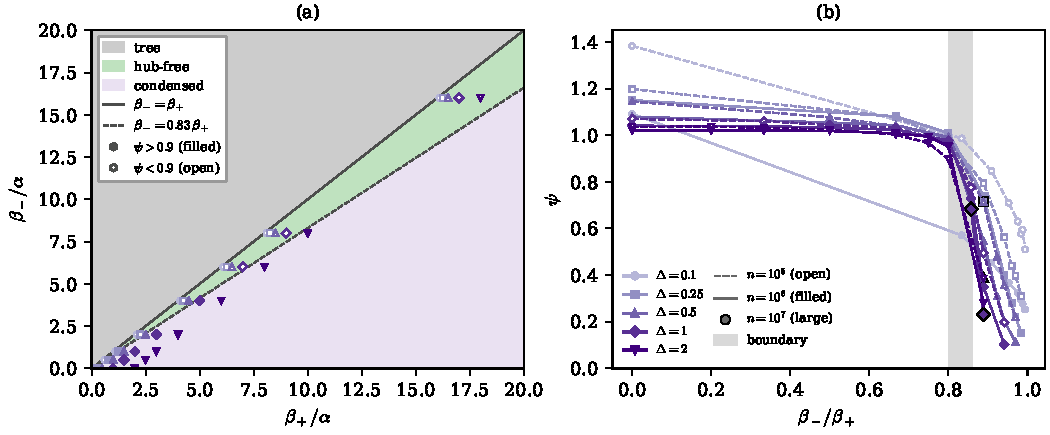
\includegraphics[width=\textwidth]{fig-phase.pdf}
\caption{Phase diagram of rule (w) from the triangle-cluster order parameter
$P_\triangle$. (a) The plane of turnover $\beta_-/\beta_+$ and deletion
$\alpha_-/\alpha_+$, at net closure per arrival $\Delta=1$ (circles) and
$\Delta=1/2$ (squares). A symbol is filled when $P_\triangle$ rises between
$n=10^5$ and $10^6$, or exceeds $0.9$ at $10^6$, and open when it falls; seeds
per point in Table~S1 of the Supplemental Material \cite{supp}. Shades: condensed (purple), dispersed
(green) and tree (grey, $\beta_-\ge\beta_+$) regimes. Dashed line: the fit of
Eq.~\eqref{eq:bnd} to the $\Delta=1$ boundary. (b) $P_\triangle$ against
$\beta_-/\beta_+$ at $\Delta=1$, without deletion (purple) and with
$\alpha_-=\alpha_+/2$ (orange), for $n=10^4$ (dotted lines, open circles),
$10^5$ (dashed lines, open squares) and $10^6$ (solid lines, filled triangles).
Means over 1--6 seeds, and over 64, 32 and 16 more at $\beta_-/\beta_+=0.70$--$0.80$,
$\alpha_-=0$; error bars, one standard error.}
\label{fig:phase}
\end{figure*}


Condensation is a statement about where the triangles go, and the order
parameter should say so without a choice of scale. Call two triangles adjacent
when they share a link, and a \emph{triangle cluster} a connected set of
adjacent triangles: a 3-clique community in the language of clique percolation
\cite{derenyi2005,palla2005}. Every closure creates at least one triangle, so
the clusters record where the closures went. Let $T$ be the number of
triangles in the network and $T_{\max}$ the number of triangles in its largest
triangle cluster. We take as order parameter the fraction of all triangles in
the largest cluster,
\begin{equation}
  P_\triangle=\frac{T_{\max}}{T},
  \label{eq:fT}
\end{equation}
the analogue for triangles of the fraction $P$ of nodes in the giant
component, together with the fractions $P_\bullet$ and $P_{\bullet{-}\bullet}$ of
all nodes and links that this cluster spans. If the triangles are scattered
over finite clusters, $P_\triangle\to0$. If $P_\triangle$ stays finite they
percolate, and $P_\bullet$ separates extended percolation, $P_\bullet$ finite,
from condensation, $P_\bullet\to0$. The clusters are found by union-find over
links, joining the three links of every triangle.

We ran rule (w) at $\Delta=1/2$ and $1$, at $\alpha_-/\alpha_+=0$ and $1/2$,
for $\beta_-/\beta_+$ from $0$ to $0.95$ and $n=10^4$, $10^5$, $10^6$, refined
the turnover near the boundary in steps of $0.02$, and scanned
$\alpha_-/\alpha_+=0.1$--$0.9$ at $\Delta=1$ (Fig.~\ref{fig:phase}). At small
turnover $P_\triangle$ rises to one with $n$; at large turnover it falls below
$10^{-3}$ at $10^6$. We call a point condensed when $P_\triangle$ rises between
$10^5$ and $10^6$ (or exceeds $0.9$) and dispersed when it falls. Along every
line of fixed $\Delta$ and $\alpha_-/\alpha_+$ the label changes once, which
brackets the boundary (Table~S1 of the Supplemental Material \cite{supp}). At
$\Delta=1$ the brackets are $0.76$--$0.78$, $0.88$--$0.90$ and $0.90$--$0.95$
at $\alpha_-/\alpha_+=0$, $0.5$ and $0.8$; at $\alpha_-/\alpha_+=0.9$ every
turnover up to $0.95$ is condensed. At $\Delta=1/2$ they are $0.72$--$0.74$ and
$0.88$--$0.90$ at $\alpha_-/\alpha_+=0$ and $0.5$. Away from $\alpha_-=0$ the
brackets rest on this criterion alone, with one or two seeds at $10^6$, and
carry the caveat discussed next.

A trend between $10^5$ and $10^6$ cannot tell a dispersed point from one that
condenses later, since without opening condensation follows a long plateau
(Sec.~\ref{sec:condensed}). We therefore followed $\beta_-/\beta_+=0.70$--$0.85$
at $\Delta=1$, $\alpha_-=0$ along single trajectories to $n=10^7$, and to
$3\times10^7$ at $0.78$ (Fig.~S1 and Table~S3 of Ref.~\cite{supp}). At $0.76$,
$P_\triangle$ is flat between $10^5$ and $10^6$ ($0.140\pm0.014$ and
$0.137\pm0.019$ over 32 and 16 seeds) and then rises to $0.30$ at $10^7$: it
condenses late. At $0.80$ and $0.85$, $P_\triangle\le10^{-4}$ at $10^7$ and
$T/n$ still decreases by $8$--$9\%$ per decade. At $0.78$ the precursors follow
those at $0.76$ about a decade later: $T/n$ levels off and rises slightly
between $10^7$ and $3\times10^7$, and the share of links among the $1\%$
highest-degree nodes reaches $0.31$ and $0.42$, against $0.36$ at $0.76$ and
$10^7$. Yet $P_\triangle$ keeps falling, to $2\times10^{-4}$ at
$3\times10^7$, while at $0.76$ it stays above $0.03$ at every size. The boundary thus
lies between $0.76$ and $0.78$ up to these sizes, and the precursors at $0.78$
suggest that it may drift to larger turnover at larger $n$. Near it, the scaled
variance $n\,{\rm var}(P_\triangle)$ over 16 to 64 seeds peaks at $0.76$ and
grows with $n$, and a Binder-type cumulant dips from $0.66$ to below $0.45$
(Table~S2 of Ref.~\cite{supp}). Three sizes support no scaling collapse, and the
data neither show a discontinuity nor establish a continuous transition.

Deletion moves the boundary towards $\beta_-=\beta_+$, with the uncertainty of
these brackets. At $\Delta=1$ a fit to
the midpoints of the nine brackets at $\alpha_-/\alpha_+=0$--$0.8$ gives
\begin{equation}
  1-\Bigl(\frac{\beta_-}{\beta_+}\Bigr)_c\simeq0.223\Bigl(1-\frac{\alpha_-}{\alpha_+}\Bigr),
  \label{eq:bnd}
\end{equation}
which misses two brackets by at most $0.006$. It vanishes at $\alpha_-=\alpha_+$
by construction, and the brackets there are too wide to tell whether the
dispersed regime closes. The shift is not an effect of density or of the rates
per surviving node: at $\alpha_-/\alpha_+=0.5$ the boundary is at $0.89$ for
both $\Delta=1/2$ and $1$, whereas at the same $\langle k\rangle\approx3$ it is
at $0.73$ ($\Delta=1/2$, $\alpha_-=0$) and $0.875$ ($\Delta=1$,
$\alpha_-/\alpha_+=0.3$). We have not identified its mechanism.

There are thus three regimes. In the \emph{condensed} phase one triangle
cluster, made of closure links, holds essentially all the triangles and spans
a vanishing fraction of the nodes (Sec.~\ref{sec:condensed}). In the
\emph{dispersed} regime the triangles are extensive but stay in finite
clusters up to $n=10^7$ (Sec.~\ref{sec:hubfree}). In the \emph{tree} phase,
$\beta_-\ge\beta_+$, there are $O(1)$ triangles (Sec.~\ref{sec:tree}). Their
degree distributions are in Fig.~\ref{fig:degree}b.


\begin{figure*}[t]
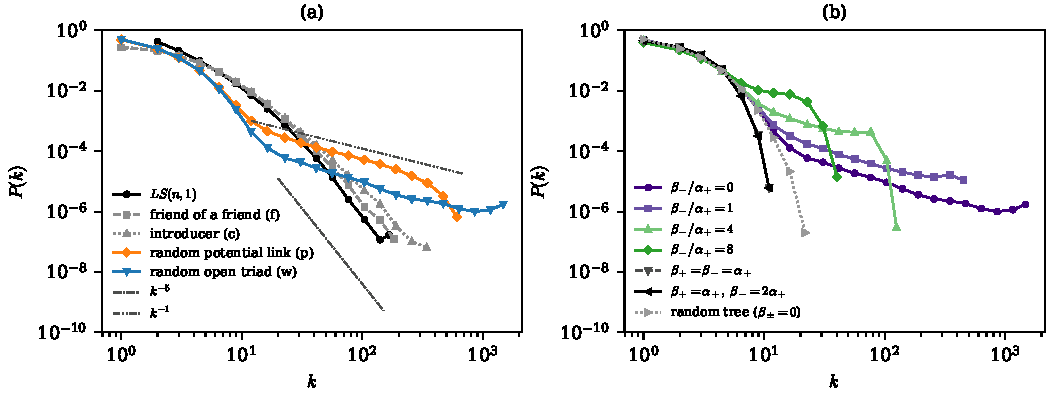
\includegraphics[width=\textwidth]{fig-degree.pdf}
\caption{Degree distributions in logarithmic bins, $n=10^6$. (a) The closure
rules without opening at $\langle k\rangle=4$ ($u=1/2$). Reference lines:
$k^{-5}$, the mean-field tail of rule (f) and $LS(n,1)$, and $k^{-1}$, a guide
to the slow decay of rule (w) before its maximum at $k\sim\sqrt n$. (b) Rule
(w) across the phase diagram at $\langle k\rangle=4$: $\beta_-/\beta_+=0$ and
$0.5$ (condensed, purple), $0.8$ and $0.89$ (dispersed, light and dark green);
at the tree transition $\beta_-/\beta_+=1$ (dashed) and in the tree phase,
$\beta_-/\beta_+=2$ (black), both at $\beta_+=\alpha_+$; and the uniform random
tree, $\beta_\pm=0$ (dotted). One network per curve.}
\label{fig:degree}
\end{figure*}

%=====================================================================
\section{The condensed phase}
\label{sec:condensed}

\subsection{Without opening: a dense core}

\begin{table}[b]
\caption{Rules without opening at $u=1/2$ ($\langle k\rangle=4$), $n=10^6$.
$b$: age exponent, fitted over $10^2<n_i<10^5$; $b_{\rm MF}=qu/2$;
$\mathcal T$: transitivity; $\bar C$: mean local clustering; $r_k$: degree
assortativity \cite{newman2002}; $\phi(\sqrt n)$: club fraction of the $\sqrt n$ highest-degree
nodes; $\rho$: link density among them. $^{\rm a}$With a core of old hubs and a
second maximum at $k\sim\sqrt n$, $k_i(n_i)$ is not a power law for rule (w).}
\label{tab:rules}
\begin{ruledtabular}
\begin{tabular}{lccccccc}
rule & $b$ & $b_{\rm MF}$ & $k_{\max}$ & $\mathcal T$ & $\bar C$ & $r_k$ & $\phi(\sqrt n)\ (\rho)$\\
\hline
$LS(n,1)$ & 0.27 & 1/4 & 169 & 0.25 & 0.69 & 0.05 & 0.001 (0.002)\\
(f) & 0.31 & 1/4 & 203 & 0.24 & 0.37 & 0.28 & 0.002 (0.008)\\
(c) & 0.37 & 1/2 & 391 & 0.22 & 0.42 & 0.16 & 0.002 (0.007)\\
(p) & 0.66 & 1/2 & 684 & 0.03 & 0.02 & 0.52 & 0.026 (0.11)\\
(w) & ---$^{\rm a}$ & 1/2 & 1619 & 0.48 & 0.008 & 0.65 & 0.20 (0.81)\\
\end{tabular}
\end{ruledtabular}
\end{table}

With $\beta_-=\alpha_-=0$ the only parameter is $u=\beta_+/(\alpha_++\beta_+)$,
and $\langle k\rangle=2/(1-u)$. Under rule (w) at $u=1/2$ and $n=10^6$, the
$\sqrt n=10^3$ highest-degree nodes are linked to one another with density
$0.81$ and hold $20\%$ of all links, a share that does not shrink with $n$. Measures that do not presuppose the core size agree on
$\Theta(\sqrt n)$ nodes: between $n=10^4$ and $10^6$ the maximal $k$-core grows
as $n^{0.47}$, the densest subgraph found by greedy peeling
\cite{charikar2000} as $n^{0.50}$, and the largest set of top-ranked nodes linked with density at
least $1/2$ as $n^{0.53}$. Hence $T\sim n^{3/2}$. The core seeds the giant
triangle cluster, which holds $P_\triangle=0.99996$ of the triangles on
$P_\bullet\sim n^{-0.45}$ of the nodes (Fig.~\ref{fig:cluster}a): the core and
the peripheral nodes tied to it by closures. Tagging each link with its origin,
the cluster contains $99.4\%$ of the closure links and $1\%$ of the arrival
links. The transitivity stays near $0.5$ while the mean local clustering
vanishes (Table~\ref{tab:rules}), and the degree distribution has a second
maximum at $k\sim\sqrt n$ (Fig.~\ref{fig:degree}a).

The hub degree follows from the core's own triads. Once triads centred in the
core dominate the census, a core node $a$ is an endpoint of a closure with
probability $w_a/W$. Here $w_a\simeq\rho\sqrt n\,K$ counts the open triads
through its $\rho\sqrt n$ core neighbours, and $W\simeq\sqrt n\,K^2/2$. Hence
$n\,dK/dn\simeq2\rho r_+n/K$ and
\begin{equation}
  K^2\simeq c\,r_+\,n ,
  \label{eq:K}
\end{equation}
with $c$ of order $4\rho$. The data give $k_{\max}^2/(r_+n)=2.5$--$2.8$ for
$u=0.3$--$0.6$ at $n=10^6$; between $10^5$ and $10^7$, $k_{\max}\sim n^{0.48}$,
close to but slightly below $\sqrt n$.

\begin{figure*}[t]
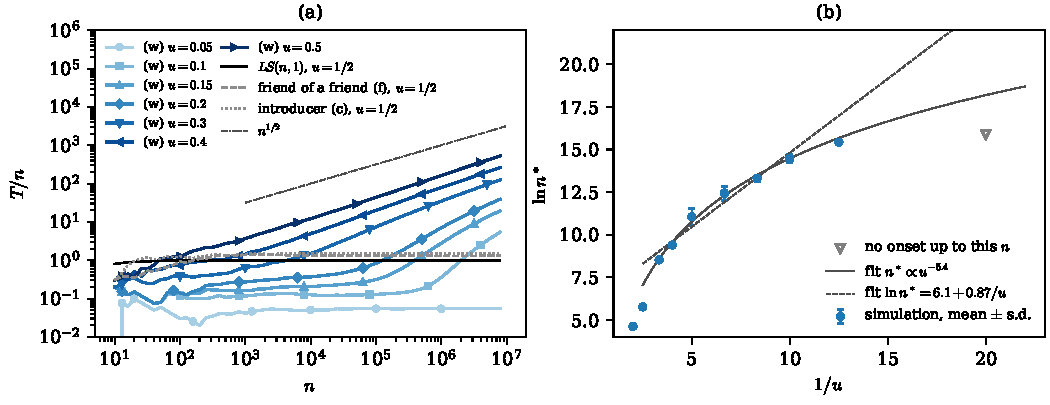
\includegraphics[width=\textwidth]{fig-transition.pdf}
\caption{Condensation without opening. (a) Triangles per node $T/n$ along
single trajectories to $n=10^7$: rule (w) at $u=0.05$--$0.5$ (blue lines with
symbols, light to dark), and the local rules and $LS(n,1)$ at $u=1/2$ (grey and black).
Dash-dotted line, $n^{1/2}$. (b) Onset size $n^*$, the first $n$ at which $T/n$
reaches twice its plateau minimum, mean and standard deviation over 5--6 seeds
for $0.08\le u\le0.25$, two at $u=0.05$ and one otherwise. Lines are fits over
$0.08\le u\le0.3$: a power law (solid) and an essential singularity (dashed).
At $u=0.05$, one trajectory condenses at $n\approx5\times10^7$ (circle) and the
other has no onset up to that size (triangle).}
\label{fig:transition}
\end{figure*}

\paragraph*{Onset.}
At small $u$ a long plateau, with constant $T/n$, precedes the condensate and
ends abruptly (Fig.~\ref{fig:transition}a). The plateau level itself falls with
$u$, from $0.46$ at $u=0.25$ to $0.05$ at $u=0.05$, so we take the onset size
$n^*$ as the first $n$ at which $T/n$ reaches twice its plateau minimum. Then
$\ln n^*=14.2$, $13.4$, $11.2$, $9.3$ at $u=0.08$, $0.10$, $0.15$, $0.25$,
with seed-to-seed spread $0.2$--$0.4$ (Fig.~\ref{fig:transition}b). Over
$0.08\le u\le0.3$ a power law, $n^*\propto u^{-4.0}$, and an essential
singularity, $\ln n^*=7.1+0.59/u$, fit equally well (rms $0.25$ and $0.22$ in
$\ln n^*$), but they part at smaller $u$: at $u=0.05$ they predict
$n^*\approx8\times10^6$ and $1.6\times10^8$. Of two trajectories followed to
$5\times10^7$, one condenses at $n^*\approx5\times10^7$ ($\ln n^*=17.7$) and the
other has not yet, although its $T/n$ is rising. The onset thus grows faster
than the power law and, from one trajectory, no faster than the essential
singularity. Condensation occurs down to $u=0.05$ at least; the data do not
decide whether it occurs at every $u>0$ or below a threshold $u_c<0.05$.

\paragraph*{Mechanism.}
A hub of degree $K$ is the centre of $\sim K^2/2$ triads, and each closure
centred on it raises the degree of two of its neighbours. A two-variable
caricature captures this feedback, which the mean field of Eq.~\eqref{eq:mf}
misses. Let $s=\sum_{c\in\partial a}k_c$ be the summed degree
of the neighbours of a hub $a$ of degree $K$, $x=\ln n$, and
$\epsilon=r_+/\bar w$, with $\bar w=W/n$ the open triads per node. The hub is an
endpoint of a closure with probability $w_a/W\simeq s/W$, so
$K'=n\,dK/dn\simeq\epsilon s$. It is the centre of about $K^2/2$ open triads,
each closure of which adds one to the degree of two of its neighbours, so
$s'\gtrsim\epsilon K^2$. Hence $K''\simeq\epsilon^2K^2$, which blows up at a
finite $x^*\sim\epsilon^{-1}K_0^{-1/2}$ for any $\epsilon>0$. The blow-up stops
when the core dominates $W$, which gives Eq.~\eqref{eq:K}. The caricature
explains why there is no threshold in sight, but not the form of $n^*(u)$. On
the plateau, $\ln n^*$ against $1/\epsilon$ fits worse (rms $0.56$) than either
form above.

\subsection{With deletion: a steady state}
\label{sec:deletion}

In a growing network the hubs are the oldest nodes, so the condensate might be a
relic of the first arrivals. Deletion separates the two, since every node is
eventually removed. The network holds $n\propto(\alpha_+-\alpha_-)t$ nodes,
each deleted at rate $\alpha_-/n$, so a node that arrived when a fraction $s$
of all arrivals had taken place survives with probability
$s^{\alpha_-/(\alpha_+-\alpha_-)}$, and the median $s$ of the survivors is
$2^{-(1-\alpha_-/\alpha_+)}$.

We ran rule (w) without opening at $u=0.3$ and $1/2$ and
$\alpha_-/\alpha_+=0$--$0.95$, up to $n=10^6$. The condensate survives at every
deletion rate. At $u=1/2$ and $n=10^6$, $P_\triangle\ge0.9998$, the cluster
holds $95$--$99\%$ of the closure links and at most $1\%$ of the arrival links
(from the link tags), and
$P_\bullet\sim n^{-0.45}$ as without deletion (Fig.~\ref{fig:cluster}a). The
largest degree still grows as $\sqrt n$: $k_{\max}=71$, $268$, $986$ at
$n=10^4$, $10^5$, $10^6$ for $\alpha_-=0.95\,\alpha_+$. At $u=0.3$ deletion
delays the onset but does not prevent it. The condensate is young: the median
arrival fraction $s$ of the $\sqrt n$ highest-degree nodes is $0.001$ without
deletion and $0.34$, $0.90$, $0.96$ at $\alpha_-/\alpha_+=0.5$, $0.9$, $0.95$,
against $0.71$, $0.93$, $0.97$ for a random surviving node. At strong deletion
the hubs are as young as the population. The condensate is a steady state:
core nodes are deleted, and census closure promotes others from the periphery
to replace them.

\subsection{With opening: a sparse cluster}

\begin{figure*}[t]
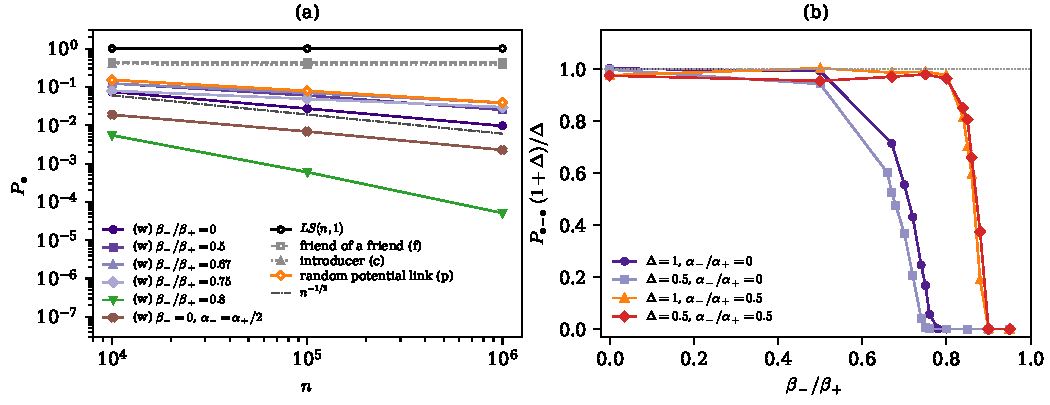
\includegraphics[width=\textwidth]{fig-cluster.pdf}
\caption{The largest triangle cluster. (a) Fraction $P_\bullet$ of the nodes that it
spans, against $n$: rule (w) at $\Delta=1$ without deletion for
$\beta_-/\beta_+=0$--$0.75$ (condensed, purple, dark to light) and $0.8$
(dispersed, green); rule (w) at $\beta_-=0$, $\Delta=1$, $\alpha_-=\alpha_+/2$
(brown crosses); and, without opening at $u=1/2$, rule (p) (orange diamonds),
the local rules (grey) and $LS(n,1)$ (black). Dash-dotted line, $n^{-1/2}$.
Means over two seeds at $n=10^4$ and one or two at larger $n$. (b) Measured
fraction of the closure links that lie inside the cluster, from the link-origin
tags, against $\beta_-/\beta_+$ at $n=10^6$ (one seed), for $\Delta=1$ and
$1/2$ with $\alpha_-/\alpha_+=0$ and $0.5$. Dotted line: all closure links.}
\label{fig:cluster}
\end{figure*}

Opening hits a link in proportion to its triangles, so it falls mainly on the
core, which thins out: at $\Delta=1$ and $n=10^6$ the share of links among the
$\sqrt n$ richest nodes falls from $0.20$ to $0.02$ and $0.005$ at
$\beta_-/\beta_+=0.5$ and $0.67$. The triangle cluster does not dissolve. At
$\beta_-/\beta_+=0.5$, $P_\triangle=0.96$, $0.98$, $0.996$ at $n=10^4$, $10^5$,
$10^6$, and the cluster holds $97\%$ of the closure links
(Fig.~\ref{fig:cluster}b). It spreads over more nodes, but their share still
vanishes, $P_\bullet\sim n^{-\lambda}$ with $\lambda=0.44$, $0.35$, $0.25$ at
$\beta_-/\beta_+=0$, $0.5$, $0.67$ (Fig.~\ref{fig:cluster}a), and the second
maximum of the degree distribution disappears (Fig.~\ref{fig:degree}b).
Approaching the boundary the cluster first loses closure links and then
triangles: at $\beta_-/\beta_+=0.72$ it holds $38\%$ of them while
$P_\triangle=0.73$ (Fig.~\ref{fig:cluster}b).

%=====================================================================
\section{The dispersed regime}
\label{sec:hubfree}

Above the boundary the triangles break into finite clusters, but the closure
links still go to the nodes of highest degree. At $\Delta=1$, $\alpha_-=0$ and
$\beta_-/\beta_+=0.8$ there are $0.14$ triangles per node at $n=10^6$, while the
largest cluster spans about $50$ nodes (Fig.~\ref{fig:cluster}a, green). The share of links among the $1\%$
highest-degree nodes grows along the trajectories as in the condensed phase
(Sec.~\ref{sec:phase}), and the largest degree grows as $n^{0.25}$ at $0.80$.
These hubs form the shoulder of
$P(k)$ at $k\approx30$--$100$ (Fig.~\ref{fig:degree}b). At $\beta_-/\beta_+=0.8$
and $n=10^6$ the nodes with $k\ge30$ are $2.8\%$ of the total, and $97\%$ of the links among them come from closures,
but their mutual link density is only $0.002$ and their triangles do not
connect. The same club forms in the condensed phase, where its triangles
percolate: the regimes differ in whether the triangles among the hubs connect,
not in whether closure links gather on them.

%=====================================================================
\section{The tree phase}
\label{sec:tree}

For $\beta_-\ge\beta_+$ nearly every triangle is opened soon after it forms,
and two times in three the opening removes a link at the centre $c$, which
passes it to one of its neighbours. Under rule
(w) the centre is drawn with weight $k_c(k_c-1)$. A node therefore loses links
at a rate quadratic in its degree and gains them, as a neighbour of a centre, at
a rate linear in it. The degrees are not bounded, but their tail falls faster
than exponentially.

The data confirm this (Fig.~\ref{fig:degree}b; Table~S4 of Ref.~\cite{supp}).
At $\beta_+=\alpha_+$ the largest degree grows from $9$ at $n=10^4$ to
$12$--$14$ at $10^7$, against $24$ for the uniform random tree at $10^6$, and
$k\,P(k)/P(k-1)\approx2$ for $k\ge4$. This Poisson-like tail,
$P(k)\propto2^k/k!$, is the one expected from losses quadratic and gains linear
in $k$; its maximum grows as $\ln n/\ln\ln n$, by a factor $1.4$ over these
sizes, as measured. At $\beta_+=\beta_-$ the degree distribution is the same,
and $T=74$ and $2060$ at $n=10^4$ and $10^7$, $T\propto n^{0.50}$, as for a
critical queue. Deletion adds a service term, $3T/n$ triangles per deleted
node, which vanishes for $T\ll n$: it leaves the boundary in place and confines
$T$ at the boundary to the same $\sqrt n$ scale.

%=====================================================================
\section{Other closure rules}
\label{sec:local}

Rule (p) also condenses, although without a dense core. At $u=1/2$ its largest
triangle cluster holds $P_\triangle=0.97$, $0.98$, $0.99$ of the triangles at
$n=10^4$, $10^5$, $10^6$ and, at $10^6$, $98\%$ of the closure links (from the
link tags) on a share of the nodes that falls as $P_\bullet\sim n^{-0.29}$
(Fig.~\ref{fig:cluster}a). Its core is sparse, with density $0.1$ among the
$\sqrt n$ richest nodes, and its largest degree grows as about $n^{0.35}$:
without the $m$-fold weight of pairs sharing $m$ neighbours there is no drive
towards a clique. Its age exponent, $b=0.66$, is far from the mean-field $1/2$.

The local rules never condense. Their triangles percolate on an extended
cluster: at $u=1/2$ the largest one holds $P_\triangle=0.83$ (f) and $0.77$ (c)
of the triangles and spans $P_\bullet=0.43$ and $0.37$ of the nodes at
$n=10^6$, nearly as at $10^4$. In $LS(n,1)$ one cluster holds everything,
$P_\triangle=P_\bullet=1$. Without opening the local rules are
described by Eq.~\eqref{eq:gamma} only roughly: the age exponent $b$ is $0.31$
for (f) (mean field $1/4$) and $0.37$ for (c) (mean field $1/2$), against
$0.27$ for $LS(n,1)$ (Table~\ref{tab:rules}). With $k_{\max}\approx200$--$400$
at $n=10^6$ their tails span little more than a decade, which is too short to
call them scale-free; they are broad and fall off much faster than those of
the census rules (Fig.~\ref{fig:degree}a). With opening at
$\langle k\rangle=4$, rule (f) keeps $b=0.31$--$0.34$ up to $\beta_-/\beta_+=0.8$
and stays in the $LS(n,1)$ class, while rule (c) develops a broader tail
without concentrating links. At $\beta_+=\beta_-$ rule (f) reaches the same
critical tree as rule (w).

%=====================================================================
\section{Communities}
\label{sec:mixing}


\begin{table}[b]
\caption{Communities at $n=10^5$ (in parentheses, $n=10^4$). $B_{\rm pp}$:
groups of the planted-partition model \cite{zhang2020}; $Q$: modularity of that
partition; $S_1$: fraction of nodes in its largest group; $\bar k_s$: mean
degree outside the largest group; $B_{\rm sbm}$ and $L$: groups at the bottom
level and nontrivial levels of the nested degree-corrected SBM
\cite{peixoto2014}. Rule (w) at $\langle k\rangle=4$, three seeds: ranges of
$B_{\rm pp}$, $B_{\rm sbm}$ and $L$, means of $Q$, $S_1$ and $\bar k_s$.}
\label{tab:comm}
\begin{ruledtabular}
\begin{tabular}{lcccccc}
network & $B_{\rm pp}$ & $Q$ & $S_1$ & $\bar k_s$ & $B_{\rm sbm}$ & $L$\\
\hline
$LS(n,1)$ & 1870 (216) & 0.95 & 0.002 & 4.0 & 2435 & 9\\
(f), $u=1/2$ & 1265 (154) & 0.90 & 0.005 & 4.0 & 1863 & 7\\
(c), $u=1/2$ & 1049 (148) & 0.92 & 0.005 & 4.0 & 2128 & 9\\
(p), $u=1/2$ & 3 (8) & 0.43 & 0.94 & 36 & 3 & 1\\
(w), $\beta_-/\beta_+=0$ & 22--41 & 0.27 & 0.95 & 39 & 2--5 & 1--2\\
(w), $\beta_-/\beta_+=0.5$ & 2--35 & 0.35 & 0.90 & 25 & 3 & 1\\
(w), $\beta_-/\beta_+=0.67$ & 2--9 & 0.39 & 0.92 & 28 & 3--6 & 1--3\\
(w), $\beta_-/\beta_+=0.8$ & 2--3 & 0.43 & 0.79 & 12 & 2--4 & 1--2\\
(w), $\beta_-/\beta_+=0.89$ & 2 & 0.37 & 0.66 & 8 & 2--3 & 1--2\\
(w), $\beta_-/\beta_+=0.94$ & 1 (1) & 0 & 1 & --- & 1 & 0\\
(w), $\beta_+=\beta_-$ & 1 (1) & 0 & 1 & --- & 1 & 0\\
random tree & 1 (1) & 0 & 1 & --- & 1 & 0\\
\end{tabular}
\end{ruledtabular}
\end{table}

Triadic closure generates communities \cite{jin2001,bianconi2014}, and in
data it is hard to tell apart from community structure and homophily
\cite{asikainen2020,peixoto2022}. We fit with graph-tool
\cite{peixoto_graphtool} the planted-partition model \cite{zhang2020}, which
describes assortative groups only, and the nested degree-corrected stochastic
block model (SBM) \cite{karrer2011,peixoto2014}, which describes any mixing.
Both select the number of groups by minimum description length; on
configuration-model rewirings of our networks they find one group (once the SBM
finds two, with negligible gain). The fits are limited to $n=10^5$ by memory.

The local rules and $LS(n,1)$ split into about $10^3$ assortative groups, with
$Q=0.90$--$0.95$, a number of groups nearly proportional to $n$ and $7$ to $9$
SBM levels, a hierarchy as in Refs.~\cite{jin2001,bianconi2014} and the
footprint of local closure rather than of homophily \cite{peixoto2022}. For rules
(w) and (p) the SBM finds two to six groups with at most three levels; one group holds
$66$--$95\%$ of the nodes and the others the rich nodes, of mean degree $8$ to
$39$. This is the club and periphery that condensation implies, and that the
closure-link club of Sec.~\ref{sec:hubfree} extends into the dispersed
phase; it disappears at $\beta_-/\beta_+=0.94$. The planted-partition count is
not stable: between seeds it jumps from $2$ (club and periphery) to $20$--$40$
small groups at the same parameters, so its non-monotonic dependence on
$\beta_-/\beta_+$ is noise between two fits of nearly equal description length.

%=====================================================================
\section{Conclusions}

Once the clock is fixed the model has three parameters: $\Delta$,
$\beta_-/\beta_+$ and $\alpha_-/\alpha_+$. At $\beta_-=\beta_+$ the triangles
form a critical queue, and above it the network is a tree. Below it, under rule
(w), the closure links gather on a vanishing fraction of the nodes, a
near-clique of about $\sqrt n$ nodes without opening, which survives deletion.
Local closure rules never condense. Unlike Bose--Einstein condensation
\cite{bianconi2001} or superlinear preferential attachment
\cite{krapivsky2000}, where one node captures a finite fraction of the links,
here a growing set of nodes does.

The main open question is whether the dispersed regime survives as
$n\to\infty$. Without opening the onset of condensation recedes quickly as the
closure rate decreases, and above the boundary the closure links still gather
on the hubs up to $n=10^7$. A correlated
theory of this club, with opening as a loss that grows with its triangles,
would decide it and give the onset $n^*(u)$ and the order of the transition.

\begin{acknowledgments}
All code is available at Ref.~\cite{code}.
The calculations were assisted by Claude Opus~5, an AI assistant developed by Anthropic. Nodes \& Links Ltd
provided support in the form of salary for Alexei Vazquez but did not have any additional role in the conceptualization of the study, the
analysis, the decision to publish or the preparation of the manuscript.
\end{acknowledgments}

\begin{thebibliography}{99}
\bibitem{granovetter1973} M. S. Granovetter, The strength of weak ties, Am. J. Sociol. \textbf{78}, 1360 (1973).
\bibitem{davidsen2002} J. Davidsen, H. Ebel, and S. Bornholdt, Emergence of a small world from local interactions: Modeling acquaintance networks, Phys. Rev. Lett. \textbf{88}, 128701 (2002).
\bibitem{holme2002} P. Holme and B. J. Kim, Growing scale-free networks with tunable clustering, Phys. Rev. E \textbf{65}, 026107 (2002).
\bibitem{vazquez2003} A. Vazquez, Growing network with local rules: Preferential attachment, clustering hierarchy, and degree correlations, Phys. Rev. E \textbf{67}, 056104 (2003).
\bibitem{toivonen2006} R. Toivonen, J.-P. Onnela, J. Saram\"aki, J. Hyv\"onen, and K. Kaski, A model for social networks, Physica A \textbf{371}, 851 (2006).
\bibitem{jackson2007} M. O. Jackson and B. W. Rogers, Meeting strangers and friends of friends: How random are social networks?, Am. Econ. Rev. \textbf{97}, 890 (2007).
\bibitem{kossinets2006} G. Kossinets and D. J. Watts, Empirical analysis of an evolving social network, Science \textbf{311}, 88 (2006).
\bibitem{ahmadian2021} S. Ahmadian and S. Haddadan, The wedge picking model: A theoretical analysis of graph evolution caused by triadic closure and algorithmic implications, J. Strateg. Innov. Sustain. \textbf{16}(3), 74 (2021); arXiv:2012.01691.
\bibitem{vazquez2001} A. Vazquez, Disordered networks generated by recursive searches, Europhys. Lett. \textbf{54}, 430 (2001).
\bibitem{book} A. Vazquez, \emph{Local network growth: how simple rules drive network complexity} (Independently published, 2026), ISBN 979-8181138933.
\bibitem{jin2001} E. M. Jin, M. Girvan, and M. E. J. Newman, Structure of growing social networks, Phys. Rev. E \textbf{64}, 046132 (2001).
\bibitem{bianconi2014} G. Bianconi, R. K. Darst, J. Iacovacci, and S. Fortunato, Triadic closure as a basic generating mechanism of communities in complex networks, Phys. Rev. E \textbf{90}, 042806 (2014).
\bibitem{marsili2004} M. Marsili, F. Vega-Redondo, and F. Slanina, The rise and fall of a networked society: A formal model, Proc. Natl. Acad. Sci. USA \textbf{101}, 1439 (2004).
\bibitem{grindrod2012} P. Grindrod, D. J. Higham, and M. C. Parsons, Bistability through triadic closure, Internet Math. \textbf{8}, 402 (2012).
\bibitem{cirigliano2024} L. Cirigliano, C. Castellano, G. J. Baxter, and G. Tim\'ar, Strongly clustered random graphs via triadic closure: An exactly solvable model, Phys. Rev. E \textbf{109}, 024306 (2024).
\bibitem{korandi2016} D. Kor\'andi, Y. Peled, and B. Sudakov, A random triadic process, SIAM J. Discrete Math. \textbf{30}, 1 (2016).
\bibitem{bhat2016} U. Bhat, P. L. Krapivsky, R. Lambiotte, and S. Redner, Densification and structural transitions in networks that grow by node copying, Phys. Rev. E \textbf{94}, 062302 (2016).
\bibitem{lambiotte2016} R. Lambiotte, P. L. Krapivsky, U. Bhat, and S. Redner, Structural transitions in densifying networks, Phys. Rev. Lett. \textbf{117}, 218301 (2016).
\bibitem{supp} See Supplemental Material at [URL] for per-triad rates (Sec.~S1), the boundary brackets (Table~S1), seed statistics (Table~S2), trajectories to $n=10^7$ (Fig.~S1, Table~S3) and the tree phase (Table~S4).
\bibitem{derenyi2005} I. Der\'enyi, G. Palla, and T. Vicsek, Clique percolation in random networks, Phys. Rev. Lett. \textbf{94}, 160202 (2005).
\bibitem{palla2005} G. Palla, I. Der\'enyi, I. Farkas, and T. Vicsek, Uncovering the overlapping community structure of complex networks in nature and society, Nature \textbf{435}, 814 (2005).
\bibitem{newman2002} M. E. J. Newman, Assortative mixing in networks, Phys. Rev. Lett. \textbf{89}, 208701 (2002).
\bibitem{charikar2000} M. Charikar, Greedy approximation algorithms for finding dense components in a graph, in \emph{Approximation Algorithms for Combinatorial Optimization}, LNCS Vol.~1913 (Springer, Berlin, 2000), p. 84.
\bibitem{zhang2020} L. Zhang and T. P. Peixoto, Statistical inference of assortative community structures, Phys. Rev. Research \textbf{2}, 043271 (2020).
\bibitem{peixoto2014} T. P. Peixoto, Hierarchical block structures and high-resolution model selection in large networks, Phys. Rev. X \textbf{4}, 011047 (2014).
\bibitem{asikainen2020} A. Asikainen, G. I\~niguez, J. Ure\~na-Carri\'on, K. Kaski, and M. Kivel\"a, Cumulative effects of triadic closure and homophily in social networks, Sci. Adv. \textbf{6}, eaax7310 (2020).
\bibitem{peixoto2022} T. P. Peixoto, Disentangling homophily, community structure, and triadic closure in networks, Phys. Rev. X \textbf{12}, 011004 (2022).
\bibitem{peixoto_graphtool} T. P. Peixoto, The graph-tool python library, figshare, doi:10.6084/m9.figshare.1164194 (2014).
\bibitem{karrer2011} B. Karrer and M. E. J. Newman, Stochastic blockmodels and community structure in networks, Phys. Rev. E \textbf{83}, 016107 (2011).
\bibitem{bianconi2001} G. Bianconi and A.-L. Barab\'asi, Bose-Einstein condensation in complex networks, Phys. Rev. Lett. \textbf{86}, 5632 (2001).
\bibitem{krapivsky2000} P. L. Krapivsky, S. Redner, and F. Leyvraz, Connectivity of growing random networks, Phys. Rev. Lett. \textbf{85}, 4629 (2000).
\bibitem{code} \url{https://github.com/av2atgh/LocalNetworkGrowth}, directory \texttt{triadic\_closure}.
\end{thebibliography}

\end{document}
